\documentclass{article}
\usepackage{blindtext}
\usepackage{titlesec}
\usepackage{listings}
\usepackage{geometry}
\usepackage{mathtools}
\usepackage[utf8]{inputenc}
\usepackage{siunitx}
\usepackage{soul}
\usepackage{enumitem}
\usepackage{graphicx}
\usepackage{float}
\usepackage{units}
\usepackage{amsfonts}
\usepackage{graphicx}
\usepackage{amsfonts,amssymb,amsmath,hyperref}
\usepackage{color}
\usepackage{tcolorbox}
\usepackage[bottom]{footmisc}


\setlength{\parindent}{0pt}

\definecolor{codegreen}{rgb}{0.1,0.5,0.1}
\definecolor{codegray}{rgb}{0.5,0.5,0.5}
\definecolor{codepurple}{rgb}{0.58,0,0.82}
\definecolor{backcolour}{rgb}{1,1,1}
\definecolor{codemaroon}{rgb}{0.5,0,0}

\lstdefinestyle{mystyle}{
    backgroundcolor=\color{backcolour},   
    commentstyle=\color{codegreen},
    keywordstyle=\color{codemaroon},
    numberstyle=\tiny\color{codegray},
    stringstyle=\color{codepurple},
    basicstyle=\footnotesize,
    breakatwhitespace=false,         
    breaklines=true,                 
    captionpos=b,                    
    keepspaces=true,                 
    numbers=left,                    
    numbersep=5pt,                  
    showspaces=false,                
    showstringspaces=false,
    showtabs=false,                  
    tabsize=2
}

\lstset{style=mystyle}

\geometry{
 a4paper,
 total={170mm,257mm},
 left=20mm,
 top=20mm,
 }

\title{Digital Systems Design Report 1}

\author{
    Ahmad Moniri, CID:\num{00842685}
    Pranav Malhotra, CID:\num{00823617}
}
\date{4th February 2016}

\begin{document}
\begin{titlepage}
	\centering
	{\scshape\LARGE Imperial College London \par}
	\vspace{2cm}
	{\scshape\Large Real-Time Digital Signal Processing \par}
	\vspace{1cm}
	{\scshape\Large Laboratory 2\par}
	\vspace{2.5cm}
	{\Large\itshape Ahmad Moniri, CID: 00842685 \par}
	\vspace{1cm}
	{\Large\itshape Pranav Malhotra, CID: 00823617 \par}
	\vfill
% Bottom of the page
	\begin{tcolorbox}
    \centering
    Declaration: We confirm that this submission is our own work. In it, we give references and citations whenever we refer to or use the published, or
    unpublished, work of others. We are aware that this course is bound by
    penalties as set out in the College examination offences policy \\~\\
    \underline{Signed: Ahmad Moniri, Pranav Malhotra}
    \end{tcolorbox}
	{\large \today\par}
\end{titlepage}

\tableofcontents

\newpage
\section{Introduction}
In laboratory 2 of Real-Time Digital Processing, we focus on the generation of sine wave. Sine waves form the basis function of the Discrete-Fourier Transform (DFT) thus generating sine waves of precise frequencies is of great importance. There are multiple ways of generating sine wave such as using recursive algorithms, look-up tables, CORDIC\footnote{\textbf{CO}ordinate \textbf{R}otation \textbf{DI}gital \textbf{C}ompute}/Volder's algorithm, or through direct computation using in-built math functions in the compiler. The laboratory script details the use of Infinite Impulse Response (IIR) filters and look-up tables. This report will discuss the theory and practical implementations of both these methods.

\section{IIR Filter Implementation of Sine Wave Generator}
The IIR filter is used when we want to obtain a frequency response that is characteristic of poles in the z plane. A pair of complex conjugate poles in the z-plane will correspond to a peak in the frequency response.\\\\
The IIR filter is characterised by the following difference equations,
\begin{equation}
    y[n]=\sum_{l=1}^{N} a_{l}y[n-l]+\sum_{k=0}^{M} b_{k}x[n-k]
\end{equation}
In the z-domain, the IIR is characterised by the following transfer function,
\begin{equation}
    H(z) = \frac{Y(z)}{X(z)} = \frac{\sum_{b=0}^{M}b_{k}z^{-k}}{1-\sum_{l=1}^{N}a_{l}z^{-l}}
\end{equation}
In the IIR filter used in laboratory 2, we used a 2nd order filter. The coeffients were, $b_{0}=0.7071$, $a_{1}=1.4142$ and $a_{2}=-1$. Inserting this into our general equation for an IIR filter, we obtained the following transfer function,
\begin{equation}
    H(z) = \frac{0.7071}{1+0.7071z^{-1}-z^{-2}}
\end{equation}
Evaluating the poles and zeroes of the transfer function, we obtain a double zero at the origin and a pair of complex conjugate poles at $p_{1}=0.7071+0.7071i$ and $p_{2}=0.7071-0.7071i$. We notice that the poles are located on the unit circle and thus the transfer function is marginally stable. In this case, a marginally stable system is desirable. It results in a sinewave that has a constant amplitude rather than a sinewave with an amplitude that has a decaying/growing exponential envelope. Below is the frequency and phase response of the above defined IIR Filter. The shape is exactly as expected with a peak at $\pi/4$ and a phase response that is not linear. 
\begin{figure}[h]
    \centering{}
    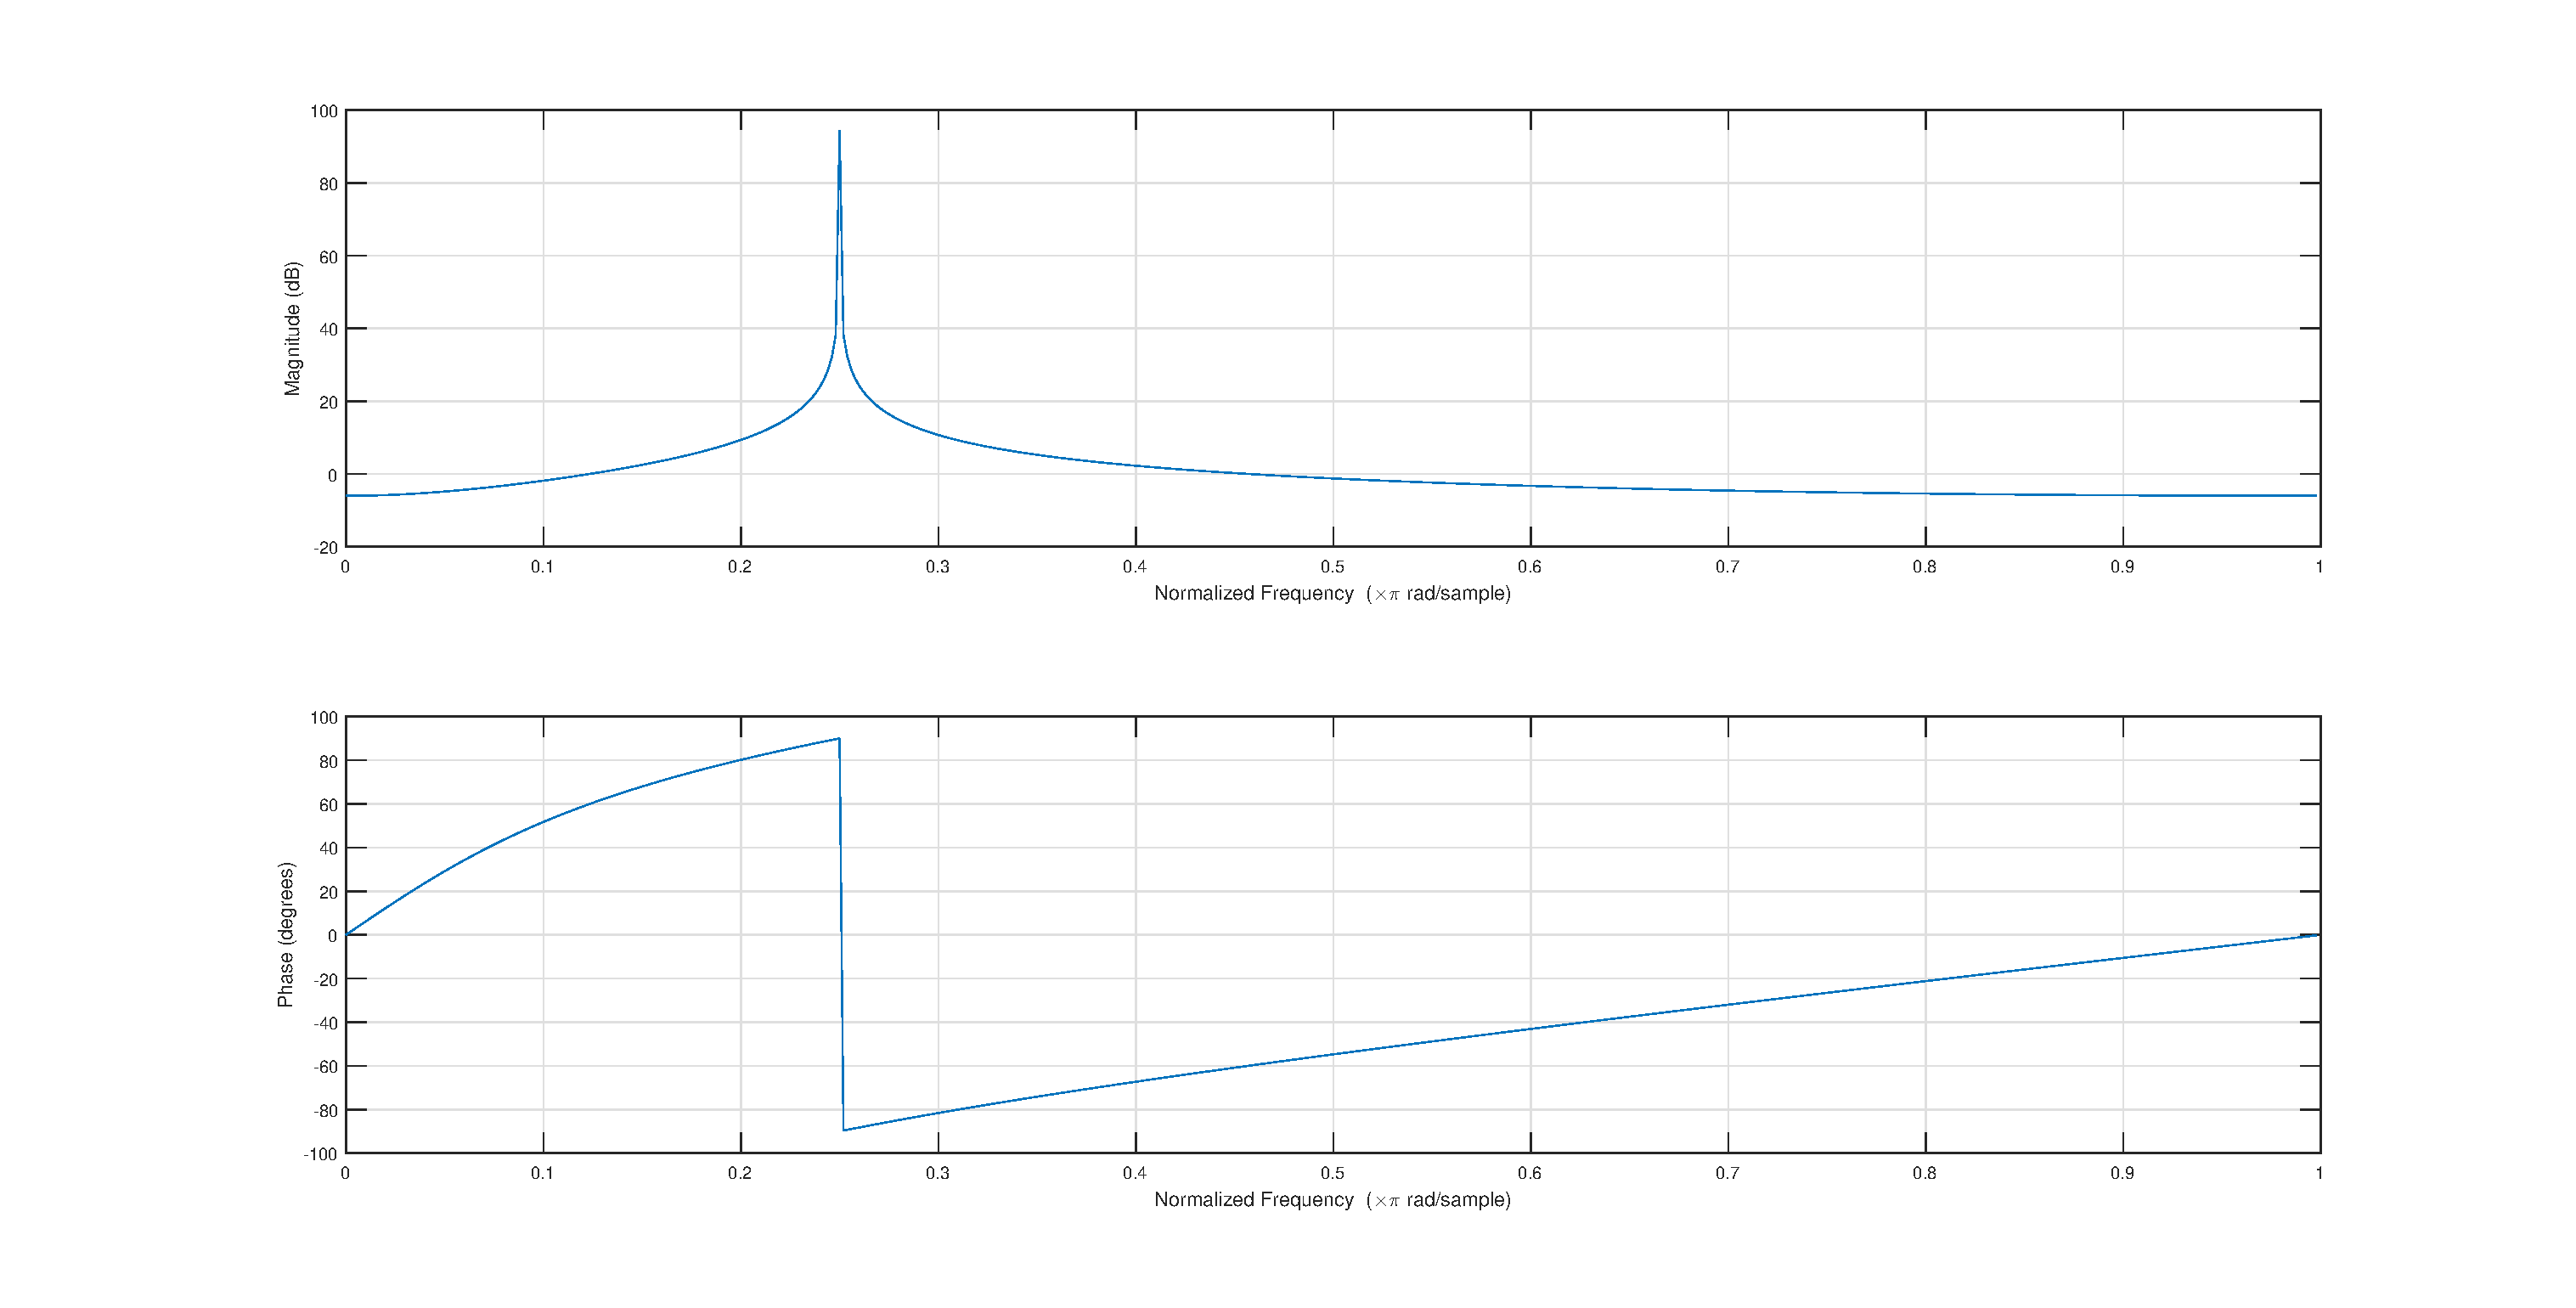
\includegraphics[scale=0.3]{frequencyresponse.eps}
    \caption{Frequency and Phase Response of above defined IIR Filter}
\end{figure}
\section{Questions in Laboratory Script for IIR Filter Implementation of Sine Wave Generator}
\textbf{Provide a trace table of {\tt sinegen} for several loops of the code. How many samples does it have to generate to complete a whole cycle?}\\\\
To generate the trace table, we need to evaluate the difference equation iteratively. To do this, we need the both the initial conditions as well as the input signal. The difference equation for the IIR filter is,
\begin{equation}
    y[n] = 1.4142y[n-1] - y[n] + 0.7071x[n]
\end{equation}
The initial conditions for the filter are,\\
\begin{equation}
    y[0] = 0,\ \ y[1] = 0,\ \ y[2] = 0
\end{equation}
And lastly, the input signal $x[n]$ is defined as,
\begin{equation}
    x = \begin{cases}
    1, \ \ \ \ x=0 \\
    0, \ \ \ \ otherwise  
  \end{cases} 
\end{equation}
Solving the difference equation, we obtain the following result,
\begin{table}[h]
\centering
\begin{tabular}{|c|c|}
\hline
\multicolumn{2}{|c|}{\textbf{Trace Table}}        \\ \hline
\textbf{Sample Number, n} & \textbf{Output Value} \\ \hline
0                         & 0.7071                \\ \hline
1                         & 1                     \\ \hline
2                         & 0.7071                \\ \hline
3                         & 0                     \\ \hline
4                         & -0.7071               \\ \hline
5                         & -1                    \\ \hline
6                         & -0.7071               \\ \hline
7                         & 0                     \\ \hline
8                         & 0.7071                \\ \hline
9                         & 1                     \\ \hline
10                        & 0.7071                \\ \hline
11                        & 0                     \\ \hline
12                        & -0.7071               \\ \hline
\end{tabular}
\caption{Trace Table for {\tt sinegen} Function}
\end{table}
It is clear that the sequence repeats itself after 8 samples. This corresponds strongly with the fact that the peak in the frequency response occurs at $\pi/4$. The frequency of the output sine wave is one-eighth the sampling frequency.\\\\
\textbf{Can you see why the output of the sinewave is currently fixed at $1 kHz$? Why does the program not output samples as fast as it can? What hardware throttles it to $1kHz$?}\\

One limitation of the IIR filter implement of the sine wave generator is that we cannot generate a sine wave with an arbitrary frequency. For the above defined IIR filter, the output sine wave will always have a frequency that is one-eighth of the sampling frequency. For this reason, with a sampling frequency of $8kHz$, the output is fixed at $1kHz$. Should we change the sampling frequency to $16kHz$, the output will be fixed at $2kHz$. Lastly, it is important to note that the codec does not support an arbitrary sampling rate. We can only implement a sampling frequency of $8kHz$, $16kHz$, $24kHz$, $32kHz$, $44.1kHz$, $48kHz$ and $96kHz$.
\newpage
\textbf{By reading through the code can you work out the number of bits used to encode each sample that is sent to the audio port?}\\


The TLV320AIC23B supports four audio-interface modes.
\begin{enumerate}
    \item Right justified
    \item Left justified
    \item I\textsuperscript{2}S mode
    \item DSP mode
\end{enumerate}
The four modes are MSB first and operate with a variable word width between 16 to 32 bits (except right-justified mode, which does not support 32 bits)\cite{audio-interface}.\\


The data manual of the TLV320AIC23 codec states that we can select a variable word width. Listed below is a snippet of the sinc.c code and refferring to line 12, we see that we have initialised the audio interface such that we use 32 bits to encode each sample that is sent to the audio port. \\

\begin{lstlisting}[language=C, frame=single, caption=Hardware Initialisation Settings]
DSK6713_AIC23_Config Config = {
                /**********************************************************************/
                /* REGISTER     FUNCTION                        SETTINGS              */ 
                /**********************************************************************/
    0x0017,     /* 0 LEFTINVOL  Left line input channel volume  0dB                   */
    0x0017,     /* 1 RIGHTINVOL Right line input channel volume 0dB                   */
    0x01f9,     /* 2 LEFTHPVOL  Left channel headphone volume   0dB                   */
    0x01f9,     /* 3 RIGHTHPVOL Right channel headphone volume  0dB                   */
    0x0011,     /* 4 ANAPATH    Analog audio path control       DAC on, Mic boost 20dB*/
    0x0000,     /* 5 DIGPATH    Digital audio path control      All Filters off       */
    0x0000,     /* 6 DPOWERDOWN Power down control              All Hardware on       */
    0x004f,     /* 7 DIGIF      Digital audio interface format  32 bit                */
    0x008d,     /* 8 SAMPLERATE Sample rate control             8 KHZ                 */
    0x0001      /* 9 DIGACT     Digital interface activation    On                    */
                /**********************************************************************/
};
\end{lstlisting}


\section{Look-Up Table Implementation of Sine Wave Generator}


The look-up table implementation of the sine wave generator is extremely simple. The look-up table consist of sampled values of 1 cycle of a sine wave. The number of samples depends on the user; a greater number of samples results in a more precise output, however it increases the space complexity of our algorithm. For this experiment, the laboratory stipulates that we have a look-up table with 256 samples. \\


As opposed to the IIR filter implementation, the look-up table allows us to form sine waves of any frequency and is not limited to sine waves with frequencies that are one-eighth the sampling frequency. This however does not mean that there is no restriction of the frequencies of the sinewaves that are generated. The look-up table implementation only allows us to generate sine waves with frequencies up to the nyquist frequency.\\ 


The sine wave is generated by outputting selected points from the look-up table. For example, if all points are sent to the output one after other, with $F_{s}=8kHz$, we obtain a sine wave with $f=31.25Hz$. However, if we were to send only every other point to the output, with $F_{s}=8kHz$, we would obtain a sine wave with $f=62.5Hz$. Similarly, we can form sine waves of any frequency using the following equation, where increment defines the difference between the index of the next point to send to the output and the index of the current point,
\begin{equation} \label{increment}
    increment= \frac{sine\_freq * SINE\_TABLE \_SIZE}{sampling\_freq}
\end{equation}


Since we are limited to only 256 samples but the sine wave we want to generate is infinite in duration, there will be a wrap around effect which is implemented through modolo division of our index by 256. Also, the if the $Increment$ that is calculated using equation (\ref{increment}) is not an integer, we will obtain an index that is also not integer. To solve this problem, we simply round the index down to obtain an integer value.
\subsection{Operation of Code}
For the look-up table implementation of the sine wave generator, we first have to generate our look up table which consists of 256 evenly spaced samples of one cycle of a sine wave. Below is the function sine\textunderscore init() that achieves this. \\
\begin{lstlisting}[language=C, frame=single, caption=Initialization of Look-Up Table]
void sine_init(void){
    /* This code will initialise our lookup table. */
    int i;
    for(i=0; i<SINE_TABLE_SIZE; i++)
        table[i]=sin(2.0*PI*i/SINE_TABLE_SIZE);
}
\end{lstlisting}

Next, we have to implement a function {\tt sinegen} that will return the sample that we send to the output. This function will make use of equation (\ref{increment}). It is important to note that we have defined both the vector table containing our sampled points and the index are defined as global variables and thus will retain their values between function calls. As mentioned above, in the case that the index is not an integer, we use the function round to obtain a value that is an integer.\\
\begin{lstlisting}[language=C, frame=single, caption=Code that Returns Value Sent to Output]
float sinegen(void){
	
    index += sine_freq*SINE_TABLE_SIZE/sampling_freq;
    if(index>SINE_TABLE_SIZE-1)
        index -= SINE_TABLE_SIZE;
		
    return(table[(int)round(index)]);
}
\end{lstlisting}

The figure below shows that the code works as expected.


\begin{figure}[h]
    \centering{}
    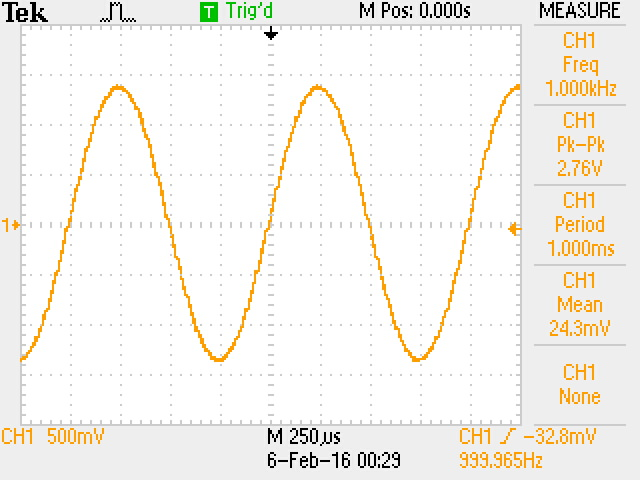
\includegraphics[scale=0.7]{8000_1000.JPG}
    \caption{$1kHz$ Sine Wave at a Sampling Frequency of $8kHz$}
\end{figure}

\newpage
\section{Questions in Laboratory Script for Look-Up Table Implementation of Sine Wave Generator}

\textbf{How to increase the resolution of the output without using a larger lookup table?}\\


There are multiple ways to increase the resolution of the output without using a larger look-up table. Firstly, we make use of the symmetry in the sine wave and only sample one-fourth of one cycle of the sine wave. Since we are still using a look-up table with 256 samples, our samples will be closer to each other. This will result in increased precision. Below are the functions {\tt sine\_init} and {\tt sinegen} that are used if we wish to increase the precision of our result,\\

\begin{lstlisting}[language=C, frame = single, caption=Functions that make use of Symmetry in Sine Wave to Increase Resolution of Output]
void sine_init(void){
	int i;
	for(i=0; i<SINE_TABLE_SIZE; i++){
		table[i] =  sin(2.0*PI*i/(4.0*SINE_TABLE_SIZE));
}

float getSineValue(int index){
    int quadrant = index/SINE_TABLE_SIZE;
    int modulo = index % SINE_TABLE_SIZE;
    
    index += sine_freq*SINE_TABLE_SIZE*4.0/sampling_freq;
    if(index>SINE_TABLE_SIZE*4.0-1)
        index -= SINE_TABLE_SIZE*4.0;
	    
    if (quadrant == 0)
        return(table[index]);
    else if (quadrant == 1)
        return(table[SINE_TABLE_SIZE-modulo-1]);
    else if (quadrant == 2)
        return(-1*table[modulo]);
    else if (quadrant == 3)
        return(-1*table[SINE_TABLE_SIZE-modulo-1]);	
    else
        return(0);
}
\end{lstlisting}
It is important to know that in this implementation, the value of index runs 0 to 1023, instead of from 0 to 255 as in the previous implementation.\\


\textbf{Discuss the limitations on upper and lower bounds of frequencies that can be generated on this system. What do you observe happening to the output as you approach what you consider to be the upper and lower limits of operation? Why?}\\



Our design was able to meet the lower bound that was stipulated in the laboratory script. There was however, significant attentuation of our signal at low freqeuencies. This is due to the high-pass filter that is present at the output of the AIC23 audio chip. The high pass filter attenuates low frequencies and is meant to remove any DC offset that the signal may contain.

\begin{figure}[h]
    \centering{}
    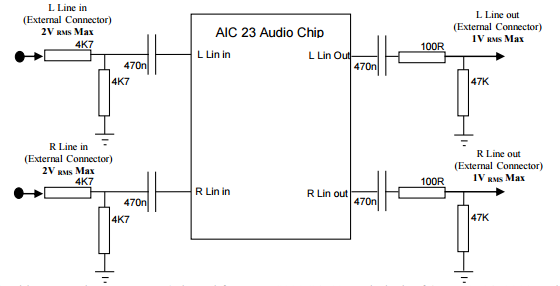
\includegraphics[scale=0.7]{AIC23.PNG}
    \caption{High-Pass Filters at Input and Output of AIC23}
\end{figure}


The scope trace below shows that the code we implemented works up to $5Hz$.

\begin{figure}[h]
    \centering{}
    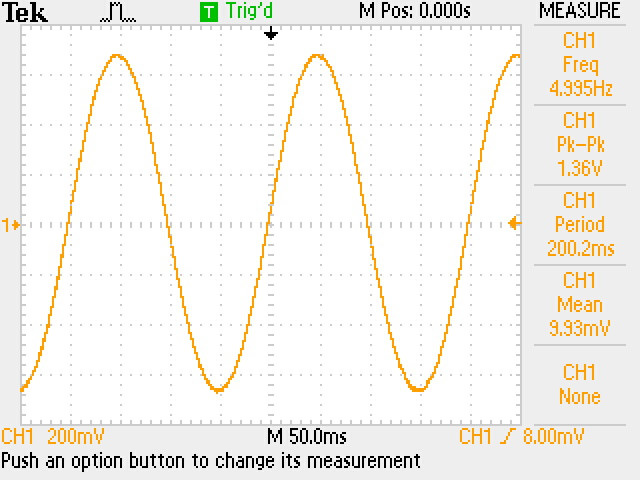
\includegraphics[scale=0.7]{8000_5.JPG}
    \caption{$5Hz$ Sine Wave at a Sampling Frequency of $8kHz$}
\end{figure}



Ideally, thee look-up table implementation of the sine wave generator should be able to generate sine waves accurately up to the nyquist frequency. This is however not the case as we observed severe distortion due to the anti-aliasing filters in the AIC23 codec. A sine wave of a single freqeuency is periodic in time and thus has a discrete spectrum in the frequency domain. This is represented by a single dirac delta function at the frequency of the sine wave. To prevent aliasing, the AIC23 codec includes a low-pass filter that will remove signals above nyquist freqeuncy. An ideal low-pass filter is represented by a rectangular function going from $-F_s$ to $F_s$. This ideal filter cannot be implemented as it would require a filter with infinite number of coefficients. However, implementing a low-pass filter with a limited number of coefficients will result in spectral leakage. When we multiply the spectrum of the low-pass filter with a dirac delta function that is located extremely close to the nyquist frequency, the resulting spectrum will go past the nyquist frequency. This results in aliasing, the very reason we implemented the anti-aliasing filter in the first place. 

\begin{figure}[h]
    \centering{}
    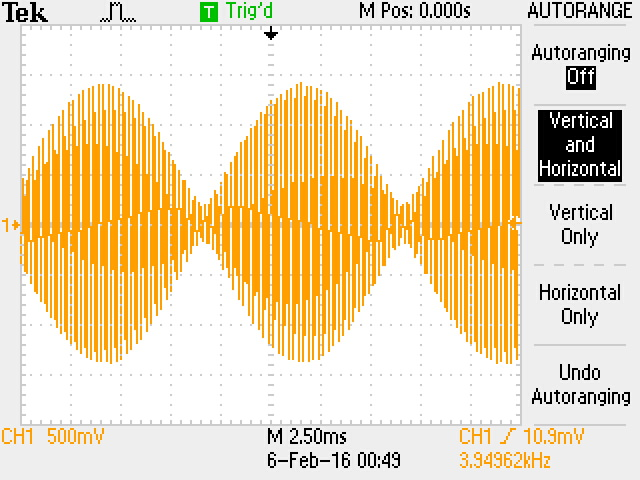
\includegraphics[scale=1]{TEK0001.JPG}
    \caption{Result of Aliasing when Generating Sine Waves near Nyquist Frequency}
\end{figure}

\newpage
\begin{thebibliography}{1}
\bibitem{audio-interface} Instruments, T. (2004). TLV320AIC23B, Stereo Audio CODEC, Data Manual. Retrieved February 04, 2016, from \url{http://www.ti.com/lit/ds/symlink/tlv320aic23b.pdf}
\end{thebibliography}


\newpage
\appendix
\section{Code}

\begin{lstlisting}[language=C, caption=Full Code Listing]
/*************************************************************************************
                    DEPARTMENT OF ELECTRICAL AND ELECTRONIC ENGINEERING
                                IMPERIAL COLLEGE LONDON 

                    EE 3.19: Real Time Digital Signal Processing
                        Dr Paul Mitcheson and Daniel Harvey

                    LAB 2: Learning C and Sinewave Generation 

                        ********* S I N E . C **********

                    Demonstrates outputing data from the DSK's audio port. 
                  Used for extending knowledge of C and using look up tables.
 *************************************************************************************
        Updated for use on 6713 DSK by Danny Harvey: May-Aug 06/Dec 07/Oct 09
                `           CCS V4 updates Sept 10
 ************************************************************************************/
/*
 *  Initialy this example uses the AIC23 codec module of the 6713 DSK Board Support
 *  Library to generate a 1KHz sine wave using a simple digital filter. 
 *  You should modify the code to generate a sine of variable frequency.
 */
/**************************** Pre-processor statements ******************************/

//  Included so program can make use of DSP/BIOS configuration tool.  
#include "dsp_bios_cfg.h"

/* The file dsk6713.h must be included in every program that uses the BSL.  This 
   example also includes dsk6713_aic23.h because it uses the 
   AIC23 codec module (audio interface). */
#include "dsk6713.h"
#include "dsk6713_aic23.h"

// math library (trig functions)
#include <math.h>

// Some functions to help with configuring hardware
#include "helper_functions_polling.h"


// PI defined here for use in your code 
#define PI 3.141592653589793

// Size of lookup table
#define SINE_TABLE_SIZE 256

/******************************* Global declarations ********************************/

/* Audio port configuration settings: these values set registers in the AIC23 audio 
   interface to configure it. See TI doc SLWS106D 3-3 to 3-10 for more info. */
DSK6713_AIC23_Config Config = {
                /**********************************************************************/
                /* REGISTER     FUNCTION                        SETTINGS              */ 
                /**********************************************************************/
    0x0017,     /* 0 LEFTINVOL  Left line input channel volume  0dB                   */
    0x0017,     /* 1 RIGHTINVOL Right line input channel volume 0dB                   */
    0x01f9,     /* 2 LEFTHPVOL  Left channel headphone volume   0dB                   */
    0x01f9,     /* 3 RIGHTHPVOL Right channel headphone volume  0dB                   */
    0x0011,     /* 4 ANAPATH    Analog audio path control       DAC on, Mic boost 20dB*/
    0x0000,     /* 5 DIGPATH    Digital audio path control      All Filters off       */
    0x0000,     /* 6 DPOWERDOWN Power down control              All Hardware on       */
    0x004f,     /* 7 DIGIF      Digital audio interface format  32 bit                */
    0x008d,     /* 8 SAMPLERATE Sample rate control             8 KHZ                 */
    0x0001      /* 9 DIGACT     Digital interface activation    On                    */
                /**********************************************************************/
};


// Codec handle:- a variable used to identify audio interface
DSK6713_AIC23_CodecHandle H_Codec;

/* Sampling frequency in HZ. Must only be set to 8000, 16000, 24000
32000, 44100 (CD standard), 48000 or 96000  */
int sampling_freq = 8000;

// Holds the value of the current sample 
float sample;

// Holds current sample number
float increment = 0;
float index = 0;
int lower_bound = 0;
int upper_bound = 0;

/* Left and right audio channel gain values, calculated to be less than signed 32 bit
 maximum value. */
Int32 L_Gain = 2100000000;
Int32 R_Gain = 2100000000;


/* Use this variable in your code to set the frequency of your sine wave 
   be carefull that you do not set it above the current nyquist frequency! */
float sine_freq = 1000.0; 

// Define look up table as global variable
float table[SINE_TABLE_SIZE];
     

/******************************* Function prototypes ********************************/
void init_hardware(void);
float sinegen(void);
void sine_init();
/********************************** Main routine ************************************/
void main()
{

	// initialize board and the audio port
	init_hardware();
	
	// initialize lookup table
	sine_init();
	
    // Loop endlessley generating a sine wave 
   while(1){
 		// Calculate next sample
 		sample = sinegen();
     	/* Send a sample to the audio port if it is ready to transmit.
           Note: DSK6713_AIC23_write() returns false if the port if is not ready */

        //  send to LEFT channel (poll until ready)
        while (!DSK6713_AIC23_write(H_Codec, ((Int32)(sample * L_Gain))))
        {};
		// send same sample to RIGHT channel (poll until ready)
        while (!DSK6713_AIC23_write(H_Codec, ((Int32)(sample * R_Gain))))
        {};
        
		// Set the sampling frequency. This function updates the frequency only if it 
		// has changed. Frequency set must be one of the supported sampling freq.
		set_samp_freq(&sampling_freq, Config, &H_Codec);	
	}

}

/******************************* init_hardware() ************************************/
void init_hardware(){
    // Initialize the board support library, must be called first 
    DSK6713_init();
    
    // Start the codec using the settings defined above in config 
    H_Codec = DSK6713_AIC23_openCodec(0, &Config);

	/* Defines number of bits in word used by MSBSP for communications with AIC23
	 NOTE: this must match the bit resolution set in in the AIC23 */
	MCBSP_FSETS(XCR1, XWDLEN1, 32BIT);
	
	/* Set the sampling frequency of the audio port. Must only be set to a supported 
	   frequency (8000/16000/24000/32000/44100/48000/96000) */
	
	DSK6713_AIC23_setFreq(H_Codec, get_sampling_handle(&sampling_freq));

}

/********************************** sinegen() ***************************************/   
float sinegen(void){
	index += SINE_TABLE_SIZE*sine_freq/sampling_freq;;

	if(index>SINE_TABLE_SIZE-1)
		index -= SINE_TABLE_SIZE;
		
    return(table[(int)round(index)]);
}

float sinegen_2(void){
    int quadrant = index/SINE_TABLE_SIZE;
    int modulo = index % SINE_TABLE_SIZE;
    
	if (quadrant == 0)
		return(table[index]);
	else if (quadrant == 1)
		return(table[SINE_TABLE_SIZE-modulo-1]);
	else if (quadrant == 2)
		return(-1*table[modulo]);
	else if (quadrant == 3)
		return(-1*table[SINE_TABLE_SIZE-modulo-1]);	
	else
		return(0);
}

float sinegen_3(void){
	index += SINE_TABLE_SIZE*sine_freq/sampling_freq;

	if(index>SINE_TABLE_SIZE-1)
		index -= 256;
	lower_bound = floor(index);
	upper_bound = ceil(index);
	
	if(lower_bound != upper_bound)
    	return(table[lower_bound] + (index - lower_bound)*(table[upper_bound]-table[lower_bound])/(upper_bound-lower_bound)); 
 
    return(table[lower_bound]); 
}



/********************************** sine_init() ***************************************/   
void sine_init(void){
	int i;
	for(i=0; i<SINE_TABLE_SIZE; i++)
		table[i]=sin(2*PI*i/SINE_TABLE_SIZE);
}

void sine_init_2(void){
	int i;
	for(i=0; i<SINE_TABLE_SIZE; i++)
		table[i] =  sin(2*PI*i/(RESOLUTION*SINE_TABLE_SIZE));
}

\end{lstlisting}

\end{document}